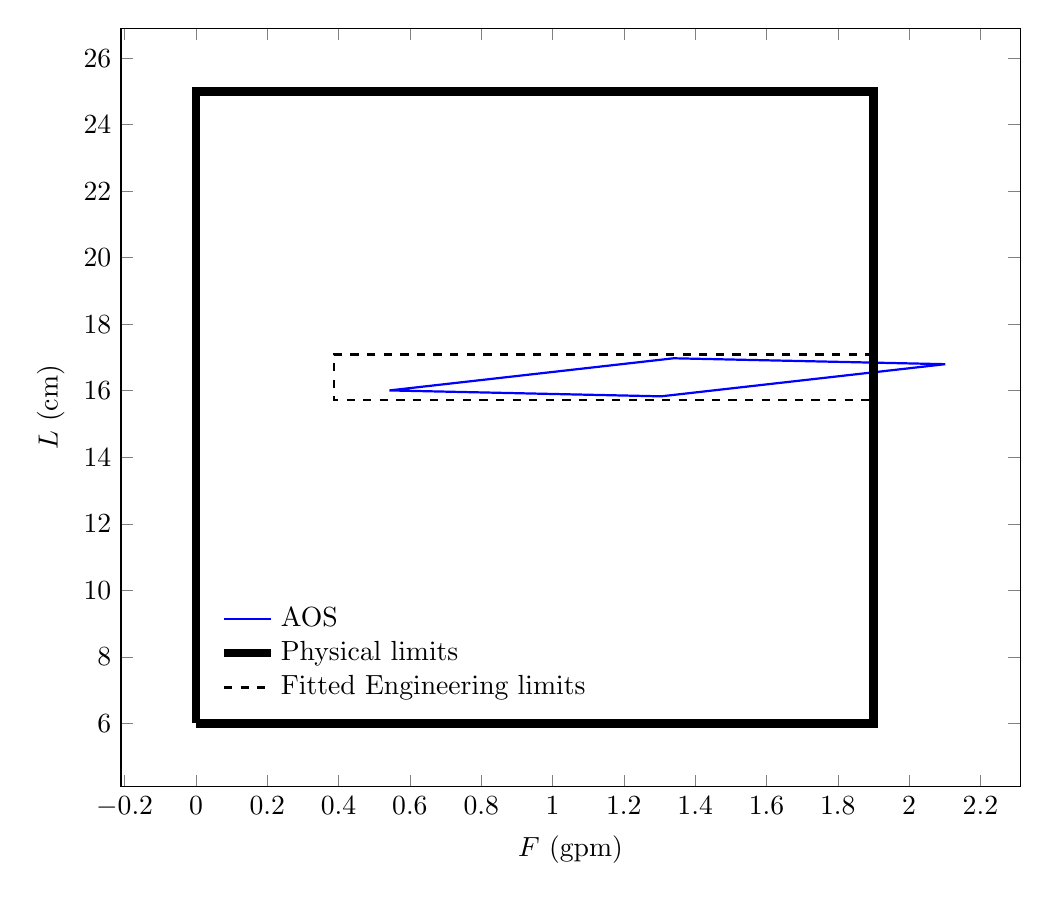
\begin{tikzpicture}
  \begin{axis}[
    width=13cm,
    xlabel=$F$~(gpm),
    ylabel=$L$~(cm),
    legend style={
      cells={anchor=west},
      at={(0.1,0.1)},
      anchor=south west,
      draw=none}]

    %AOS
    \addplot[color=blue,thick] coordinates {
      (1.3396,  16.9768)
      (2.1012,  16.7992)
      (1.3044,  15.8328)
      (0.5428,  16.0104)
      (1.3396,  16.9768)
    };
    %Physical limits
    \addplot[color=black,line width=3pt] coordinates {
      (0,  6)
      (0,  25)
      (1.9, 25)
      (1.9, 6)
      (0,  6)
    };
    %Fitted Eng limits
    \addplot[color=black,thick,dashed] coordinates {
      (1.9,      17.0912)
      (0.38696,  17.0912)
      (0.38696,  15.7184)
      (1.9,      15.7184)
      (1.9,      17.0912)
    };
    \legend{AOS,Physical limits,Fitted Engineering limits}
  \end{axis}
\end{tikzpicture}
